En esta sección se resumen los fundamentos teóricos necesarios para el resto del trabajo. Se presentan el modelo de cámara, homografías para el plano del suelo y los operadores de detección de bordes y líneas, así como la notación homogénea para rectas y el concepto de puntos de fuga.

\subsection{Modelo de cámara \emph{pin-hole} y calibración}\label{subsec:camera}

El modelo pin-hole es una aproximación matemática que describe cómo se forma una imagen
en una cámara. Como se muestra en la Fig.~\ref{fig:pinhole-model}, este modelo representa
la cámara como una caja con un pequeño orificio (\emph{pin-hole}) por donde pasa la luz.

\begin{figure}[!ht]
	\centering
	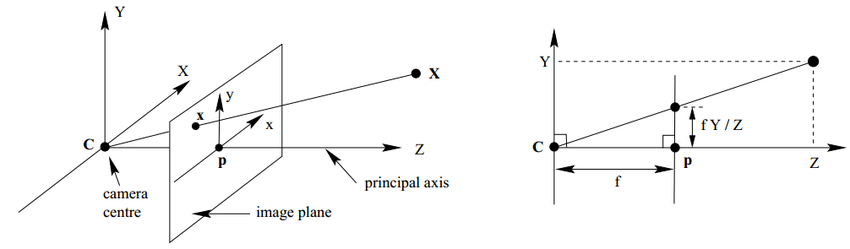
\includegraphics[width=0.99\textwidth]{img/2-mt/pinhole.png}
	\caption{Geometría del modelo de cámara pin-hole. (Imagen de \cite{hartley2003multiple}).}
	\label{fig:pinhole-model}
\end{figure}


En este modelo, un punto tridimensional \(\mathbf{X}\) del mundo se proyecta a través
del centro óptico \(\mathbf{C}\) hacia el plano de imagen, generando el punto bidimensional
\(\mathbf{x}\) en la imagen. Esta proyección es una transformación geométrica que preserva
las líneas rectas pero no las distancias ni los ángulos.


Para aplicaciones prácticas, es necesario conocer los parámetros internos de la cámara
a través del proceso calibración (calibración intrínseca). Esta calibración estima
una matriz de cámara que contiene parámetros como la distancia focal,
el punto principal y el factor de aspecto, así como coeficientes de distorsión.


Con estos parámetros, es posible normalizar las coordenadas de la imagen,
es decir, corregir las distorsiones y convertir píxeles a coordenadas métricas normalizadas.
Esto permite realizar mediciones geométricas más precisas y aplicar algoritmos
de visión por computadora con menor error \cite{hartley2003multiple}.

\subsection{Líneas y puntos en el modelo \emph{pin-hole}}\label{subsec:lines-points}

En el modelo pin-hole, tanto los puntos como las líneas pueden representarse de forma cartesiana u homogénea. La representación homogénea ofrece ventajas computacionales importantes para operaciones geométricas como intersecciones y ajustes de múltiples elementos.

\subsubsection{Representación de puntos}
Un punto en la imagen puede expresarse en coordenadas cartesianas como $(x,y)$ o en coordenadas homogéneas como $\mathbf{x}=[x,y,w]^\top$\footnote{Usualmente para convertir una coordenada cartesiana a homogenea se define $w=1$, aunque cualquier valor diferentes de $0$ puede usarse, si se usa de manera consistente.}. La representación homogénea permite trabajar con transformaciones proyectivas de forma más elegante y manejar puntos en el infinito de manera consistente.

\subsubsection{Representación de líneas}

Una línea en la imagen se representa en coordenadas homogéneas como $\ell=[A,B,C]^\top$, donde $A$, $B$ y $C$ son los parámetros de la ecuación cartesiana de la línea:
\begin{equation}
	Ax + By + C = 0
\end{equation}

\subsubsection{Relación entre líneas y puntos}
Un punto homogéneo $\mathbf{x}$ pertenece a una línea $\ell$ si y solo si:
\begin{equation}
	\ell^\top\mathbf{x} = 0
\end{equation}
Esta relación fundamental permite verificar incidencia y realizar operaciones geométricas de forma algebraica.

\subsubsection{Línea a partir de dos puntos cartesianos}\label{subsec:line-from-points}

Dados dos puntos cartesianos $(x_1,y_1)$ y $(x_2,y_2)$, la línea que los contiene se obtiene resolviendo el sistema:
\begin{equation}
	\begin{bmatrix}x_1&y_1&1\\x_2&y_2&1\end{bmatrix}\begin{bmatrix}A\\B\\C\end{bmatrix} = \mathbf{0}
\end{equation}
La solución $\ell=[A,B,C]^\top$ se encuentra calculando el espacio nulo de la matriz $\mathbf{M}$. Existen varias formas de obtener este espacio nulo, entre ellas una posible forma de hacerlo de manera simple es mediante descomposición en valores singulares (SVD) para mayor robustez numérica \cite{golub2013matrix}.

\subsubsection{Línea a partir de dos puntos homogéneos}

Si los puntos están en coordenadas homogéneas $\mathbf{x}_1$ y $\mathbf{x}_2$, la línea se calcula directamente con el producto cruz:
\begin{equation}
	\ell = \mathbf{x}_1 \times \mathbf{x}_2
\end{equation}

\subsubsection{Intersección de dos líneas}
Dadas dos líneas homogéneas $\ell_1$ y $\ell_2$, su punto de intersección se obtiene mediante:
\begin{equation}
	\mathbf{x} = \ell_1 \times \ell_2
\end{equation}

      
Sea $\mathbf{x}=[x_1,x_2,x_3]^\top$ una coordenada homogenea. Si $x_3 \neq 0$, el punto es finito y se deshomogeneiza como $(w\frac{x_1}{x_3}, w\frac{x_2}{x_3})$ . Valores $x_3 \approx 0$ indican líneas prácticamente paralelas con intersección en el infinito \cite{hartley2003multiple}.

\subsubsection{Ajuste a múltiples elementos} \label{sec:ajuste-multiples-elementos}

Para encontrar la mejor línea que pase por múltiples puntos, o el mejor punto de intersección de múltiples líneas, la solución óptima está dada por el eigenvector asociado al eigenvalor más pequeño de la matriz $\mathbf{M}$ \cite{kanatani1998statistical} que se define a continuación:
\begin{equation}
	\mathbf{M} = \sum_{i=1}^{n} w_i \mathbf{v}_i \mathbf{v}_i^\top
\end{equation}
donde $\mathbf{v}_i$ representa:
\begin{itemize}
	\item puntos homogéneos $\mathbf{x}_i$ para encontrar la línea que mejor se ajuste a los puntos
	\item líneas homogéneas $\ell_i$ para encontrar el punto de intersección de las líneas
\end{itemize} y  $w_i$ es una ponderación tal que:
\[
\sum_{i=1}^{n} w_i = 1.
\]

\subsection{Homografías en el plano del suelo}\label{subsec:homografias}

Cuando los puntos pertenecen a un mismo plano (\emph{e.g.}, el suelo),
la relación entre sus proyecciones en  dos vistas o entre el plano del
mundo   y    la   imagen   puede   modelarse    con   una   homografía
\(\mathbf{H}\in\mathbb{R}^{3\times3}\)      definida     a      escala
\cite{hartley2003multiple}. Esta  matriz permite  mapear cuadriláteros
en la imagen a cuadrados canónicos, facilitando medir y extrapolar una
retícula en la imagen.

\subsection{Bordes y líneas: Canny y Hough}\label{sec:canny-hough}

La extracción de bordes con Canny proporciona contornos estables frente a ruido mediante suavizado, gradiente y supresión no máxima \cite{canny1986edge}. La transformada de Hough detecta lineas rectas parametrizando la ecuación\[\rho=x\cos{\theta}+y\sin{\theta}\] donde $\rho$ es la distancia mínima de la recta al origen y $\theta$ es el ángulo de la normal a la recta\cite{DudaEtAl1972} {\bfseries TODO: Añadir grafica mostrando los parametros rho y theta y mostrando el resultado de aplicar Canny a una imagen}. Estas dos herramientas permiten obtener segmentos candidatos a las marcas viales de la retícula.

\subsection{Intersecciones de líneas y \emph{clustering}}\label{sec:intersections-clustering}

En escenas urbanas muchas rectas convergen hacia uno o varios puntos de fuga. Por tanto, las
intersecciones finitas tienden a concentrarse en vecindades cercanas a la línea del horizonte. Un filtrado previo por banda horizontal reduce ruido: se retienen solo las intersecciones con \(y\) dentro de una franja alrededor del horizonte estimado (véase sección~\ref{sec:vanishing-points}).


Para consolidar evidencia y atenuar datos atípicos, se agrupan las intersecciones relevantes mediante técnicas de \emph{clustering} no supervisado. Una opción práctica es el \emph{Clustering acumulativo} con umbral de distancia para dejar que los datos determinen el número de cúmulos \cite{tan2005introduction}. Los centroides de los cúmulos proporcionan estimaciones iniciales de puntos de fuga\cite{kanatani1998statistical,hartley2003multiple}.


En resumen, el proceso básico para encontrar puntos es fuga es el siguiente: (i) estimar rectas, (ii) generar intersecciones por pares, (iii) filtrar por banda cercana al horizonte, (iv) agrupar por proximidad y (v) usar los centroides de cúmulos como candidatos a puntos de fuga para la separación de haces de líneas.

\subsection{Puntos de fuga}\label{sec:vanishing-points}

Cuando proyectamos una escena del mundo real en tres dimensiones sobre un plano bidimensional,
como la película o el sensor de una cámara, se produce una transformación en la imagen.
Esta transformación, conocida como transformación proyectiva, provoca que las líneas paralelas en el mundo real,
al proyectarse en el plano de la cámara, se intersecten en un punto denominado punto de fuga.
La Fig.~\ref{fig:distorion-teo} ilustra el fenómeno de paralelismo en 3D y su proyección en 2D.

\begin{figure}[!ht]
	\centering
	\begin{subfigure}{0.4\textwidth}
		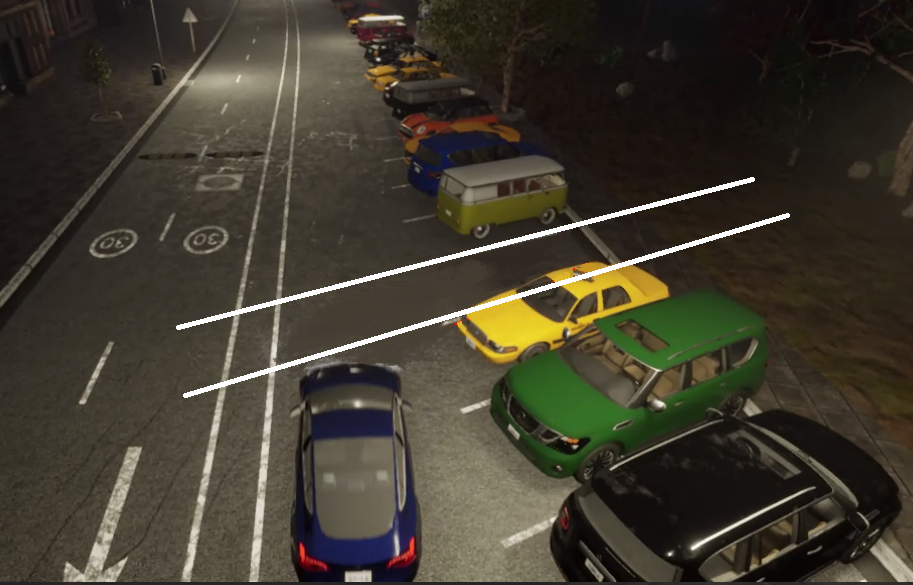
\includegraphics[width=\textwidth]{img/reticule/paralel_lines}
		\caption{Ejemplo de líneas paralelas en un escenario real en tres dimensiones.}
	\end{subfigure}
	\begin{subfigure}{0.4\textwidth}
		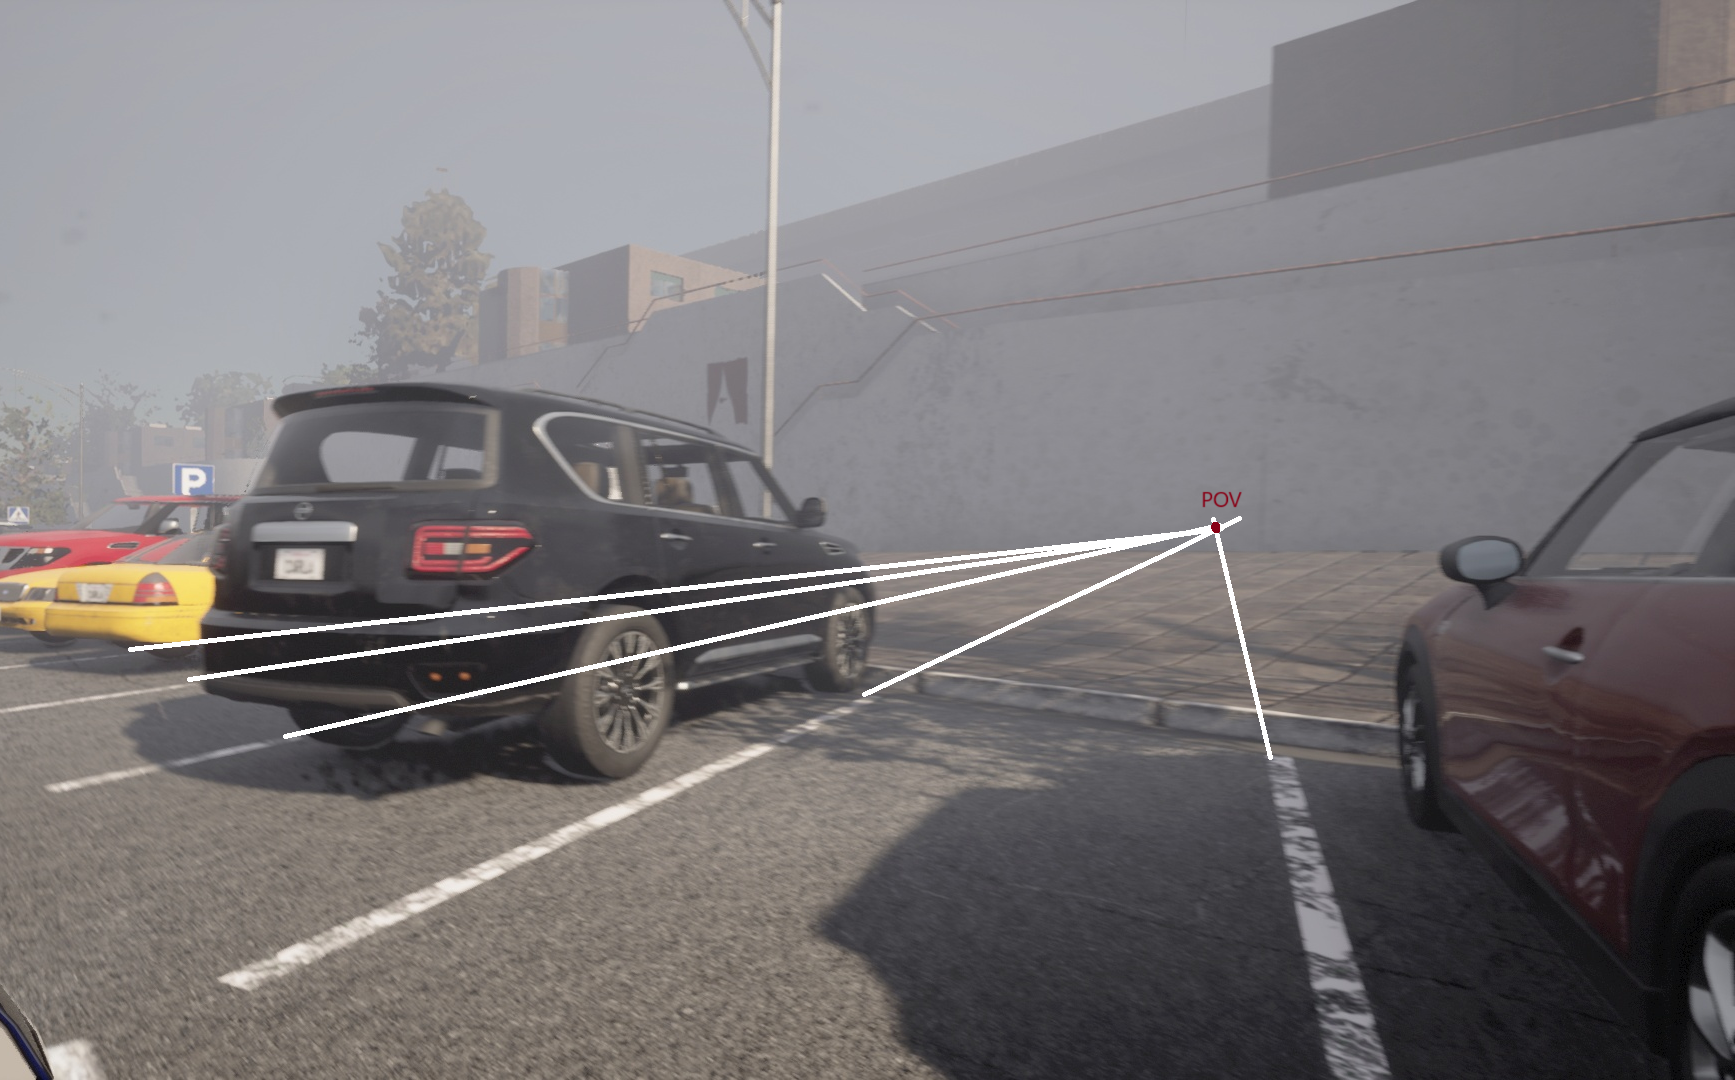
\includegraphics[width=\textwidth]{img/reticule/pov}
		\caption{Proyección de líneas paralelas en el plano de la cámara.}
	\end{subfigure}
	\caption{Paralelismo en 3D y su proyección al plano de imagen.}
	\label{fig:distorion-teo}
\end{figure}


Estimar puntos de fuga con múltiples líneas y criterios robustos reduce la sensibilidad a ruido y oclusiones
\cite{hartley2003multiple,kanatani1998statistical}. En este trabajo se emplean dos puntos de fuga para separar
las marcas de la retícula en dos conjuntos según su punto de fuga, coherentes con la geometría del estacionamiento.
